\section{概要}

\begin{frame}
  \frametitle{概要}
  % 図にする?
  プログラムを生成するプログラミング言語(=\alert{コード生成言語})の安全性を保証する研究
  \begin{itemize}
  \item<2-> 効率的なコードの生成
  \item<3-> 安全性の保証
  \item<4-> [⇒] \alert{多段階let 挿入}を安全に扱うための型システムを構築
  \end{itemize}
\end{frame}

\section{研究の背景}
\subsection{段階的計算(コード生成)}
\begin{frame}
  \frametitle{段階的計算 (Staged Computation)}
  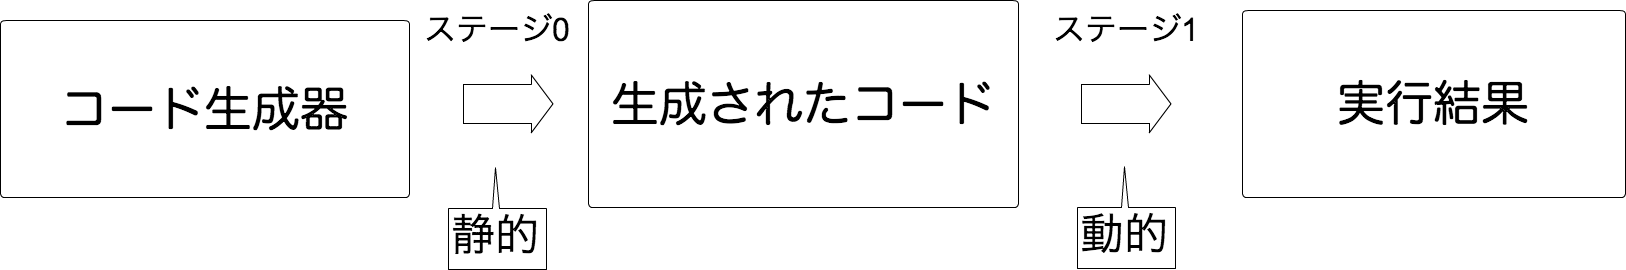
\includegraphics[clip,width=12cm]{./img/prggen.png}
  % この図を少し変更する
  \begin{itemize}
  \item コード生成ステージとコード実行ステージ
  \item[⇒] 段階的計算をサポートするプログラム言語 ⇒ コード生成言語
    % \item 生成するプログラムだけでなく,生成されたプログラムも型の整合性が静的に (生成前に) 保証される.
  \end{itemize}
\end{frame}

\subsection{コード生成の例}
\begin{frame}
  \frametitle{power関数のコード化}
  \begin{align*}
    \text{power} ~x~ ~n~ &~=~ x &\text{if} ~~n = 1 \\
                         &~~~\phantom{=}~ x * \text{power} ~x~ (n-1)~ &\text{if} ~~n > 1
  \end{align*}

  \pause
  $n = 8$に特化したコードの生成を行う
  \begin{align*}
    \text{gen\_power} ~x~ ~8~ =~ ~x~ * ~x~ * ~x~ * ~x~ * ~x~ * ~x~ * ~x~ * ~x~
  \end{align*}
  \pause
  $\text{gen\_power} ~x~ ~8~$ は$\text{power} ~x~ ~8~$ より高速
  \begin{itemize}
  \item 関数呼び出しがない
  \item 条件式がない
  \end{itemize}
\end{frame}

\subsection{段階的計算の課題}

\begin{frame}
  \frametitle{コード生成の利点と課題}
  % もっとコンパクトに

  利点
  \begin{itemize}
  \item \alert{「保守性・再利用性の高さ」}と\alert{「実行性能の高さ」}の両立
  \end{itemize}

  \pause

  課題
  \begin{itemize}
  \item パラメータに応じて,非常に多数のコードが生成される
    % \item 構文的,意味的に正しくないプログラムを生成しやすい
  \item 生成したコードのデバッグが容易ではない
  \item [⇒] \alert{コード生成の前に安全性を保証}したい
  \end{itemize}
\end{frame}

\begin{frame}
  \frametitle{従来研究}
  \begin{itemize}
  \item コード生成プログラムが,安全なコードのみを生成する事を静的に保証
    % \item<2-> let挿入等を実現する\alert{計算エフェクトを含む場合の安全性保証の研究は未整備}
  \item 安全なコード: 構文,型,変数束縛が正しいプログラム
  \end{itemize}

  \pause

  しかし\alert{多段階let挿入}等を実現する\alert{計算エフェクト}を含む場合のコード生成の安全性保証は研究途上
\end{frame}

\subsection{shift0/reset0}

\begin{frame}
  \frametitle{多段階let挿入}
  % 入れ子になったforループなどを飛び越えたコード移動を許す仕組みであり、ループ不変式の移動によって,効率的なコード生成に必要なプログラム技法

  \begin{itemize}
  \item 入れ子になったforループなどを飛び越えた\alert{コード移動}を許す仕組み
  \item ループ不変式の移動によって,\alert{効率的なコード生成}に必要なプログラミング技法
  \end{itemize}
\end{frame}

\begin{frame}[fragile]
  \frametitle{多段階let 挿入,let挿入の例}
  \begin{align*}
    & \forin{i = 0}{n} \\
    & ~~\forin{j = 0}{m} \\
    & ~~~~\magenta{\Let ~y ~= ~t ~\In} \\
    & ~~~~~~a[i][j] = b[i] + y \\
  \end{align*}

  % $\Rightarrow (\text{shift0/reset0 を付与})$

  \begin{onlyenv}<2>
    \begin{center}
      多段階let挿入\\
      $\Downarrow$
    \end{center}
    \begin{align*}
      & \magenta{\Let ~y ~= ~t ~\In} ~~~~~~~~~~\tiny{\text{--- t がi にも j にも依存しない式}} \\
      & ~~\forin{i = 0}{n} \\
      & ~~~~\forin{j = 0}{m} \\
      & ~~~~~~a[i][j] = b[i] + y \\
    \end{align*}
  \end{onlyenv}

  \begin{onlyenv}<3>
    \begin{center}
      普通のlet挿入\\
      $\Downarrow$
    \end{center}
    \begin{align*}
      & \forin{i = 0}{n} \\
      & ~~\magenta{\Let ~y ~= ~t ~\In} ~~~~~~~~~~\tiny{\text{--- t がi にのみ依存し jには依存しない式 }} \\
      & ~~~~\forin{j = 0}{m} \\
      & ~~~~~~a[i][j] = b[i] + y \\
    \end{align*}
  \end{onlyenv}

  \begin{onlyenv}<4>
    \begin{center}
      多段階let 挿入でも let挿入でもない\\
      $\Downarrow$
    \end{center}
    \begin{align*}
      & \forin{i = 0}{n} \\
      & ~~\forin{j = 0}{m} \\
      & ~~~~\magenta{\Let ~y ~= ~t ~\In} ~~~~~~~~~~\tiny{\text{--- t がi,j に依存した式 }} \\
      & ~~~~~~a[i][j] = b[i] + y \\
    \end{align*}
  \end{onlyenv}

\end{frame}

\subsection{限定継続}

\begin{frame}
  \frametitle{コントロールオペレータ}
  \begin{block}{プログラミング言語におけるプログラムを制御するプリミティブ}
    \begin{itemize}
    \item exception (例外): C++, Java, ML
    \item call/cc (第一級継続): Scheme, SML/NJ
    \item shift/reset (限定継続): Racket, Scala, OCaml
      \begin{itemize}
      \item 1989年以降多数研究がある
      \item コード生成におけるlet挿入が実現可能
        % \item shift/reset + コード生成の型システムが幾つか提案されている
      \end{itemize}
    \item \alert{shift0/reset0}
      \begin{itemize}
      \item 2011年以降研究が活発化.
      \item コード生成における\alert{多段階let挿入}が可能
      \end{itemize}
    \end{itemize}
  \end{block}
\end{frame}

%%% Local Variables:
%%% mode: japanese-latex
%%% TeX-master: "slide"
%%% End:
